\chapter{Background}

%<Paragraph> Overview of background

This chapter provides a background on molecular computation techniques.  We begin with an introduction to nanotechnology and then provide an example of how information is encoded using molecular matter.  Following this example, we introduce Adleman's molecular operators for solving an instance of {\sc Hamiltonian Path}.  The operators provide an instruction set for molecular computation, and provide the primitives for constructing molecular algorithms.

In the second half of this chapter, we provide an introduction to {\sc Satisfiability}.  We define {\sc Satisfiability} as a circuit.  We then view {\sc Satisfiability} as a language.  We also discuss practical matters related to efficiently evaluating {\sc Satisfiability}, such as how to encode input and output, and how to classify instances of {\sc Satisfiability} in the tests that we perform.

\section{On nanotechnology and construction of molecules}

%		<Paragraph> Richard Feynman [introduces] nanotechnology
		
	Richard Feynman founded the field of nanotechnology in his 1959 talk ``There's Plenty of Room at the Bottom'' \cite{feynman1959}.  Examples of applied nanotechnology include the manufacturing of graphene \cite{Stankovich_Dikin_Dommett_Kohlhaas_Zimney_Stach_Piner_Nguyen_Ruoff_2006} and DNA nanopores \cite{dnaTransistorIBMpressrelease}. Graphene consists of a planer arrangement of carbon atoms that provides desirable physical and electrical properties \cite{Stankovich_Dikin_Dommett_Kohlhaas_Zimney_Stach_Piner_Nguyen_Ruoff_2006}.  DNA nanopores use graphene to create a physical channel for reading genetic sequences \cite{Garaj2010}.  Gene sequencing technologies provide an example of applied nanotechnology \cite{Garaj2010, ionTorrent, oxfordNanopore}.  					
			%The work has driven the fields of molecular and quantum computation, VLSI circuit construction, and continues with innovative design and applications into many everyday processes.
		
%		<Paragraph> DNA substrate [builds] molecular definition
		
Smaller and cost-effective DNA sequencers provide the ability to read the contents of a gene.  Benchtop sequencers \cite{ionTorrent, oxfordNanopore} allow doctors to treat patients at the genome level from their office.  Life Technologies and Oxford Nanopore offer gene sequencers based on solid-state semiconductor technology \cite{ionTorrent, oxfordNanopore}.	

\section{Genetic encoding schemes}

%	<Paragraph> Microbiology [studies] molecular life
	Microbiology studies the interactions among organic molecules.  In this project, we explore the use of applied genetics as a means for generalized computation.  Molecular computation encodes data as sequences of DNA or RNA.  

%	<Paragraph> Each string [builds] structure from proteins
	Arbitrary encodings that represent mappings from variables to physical oligonucleotides may have undesirable structure and functionality.  Conventional techniques from molecular computation employ variable mappings from a library of oligonucleotides.
	
%	<Paragraph> Genetic alphabet [defines] life
		
%	The genetic alphabet defines a universal medium for proteins.  Each of the nucleotides (A, C, G, T, U) transcribes redundant encodings of amino acids.  Sequences of amino acids form structure as proteins.  Redundant encodings in the each amino acid permit syntax errors without a functional abnormality.  This redundant encoding structure permits mutation in the third nucleotide of each amino acid without consequence on the entire string.

%	<Paragraph> Complex molecules [contain] unique strings 
	
	An \textit{oligonucleotide} is a short string of genetic information.  There are several configurations for DNA and RNA; these include $+$RNA, $-$RNA, $+$DNA, $-$DNA, $\pm$RNA, $\pm$DNA, and +mRNA \cite{baltimore1971exp}.  The polarity of DNA denotes the direction of the genetic information.  `$+$DNA' is denoted $5'$---$3'$ and `$-$DNA' is denoted $3'$---$5'$.  We focus on $+$DNA and $-$DNA as the substrate for computational states.  The computational states, in our setting, encode candidate witnesses for {\sc Satisfiability}.


\begin{table}[htdp]
\caption{A mapping of the integers $[0,4]$ with arbitrary oligonucleotide definitions.}
\begin{center}
\begin{tabular}{|c|c|c|}
\hline
 \textbf{Integer} & \textbf{Oligonucleotide} & \textbf{Reverse-complement}\\ \hline
0 & $5'$\texttt{TCTCCC}$3'$ & $3'$\texttt{AGAGGG}$5'$ \\
1 & $5'$\texttt{AAACCC}$3'$ & $3'$\texttt{TTTGGG}$5'$ \\
2 & $5'$\texttt{GGTAAA}$3'$ & $3'$\texttt{CCATTT}$5'$ \\
3 & $5'$\texttt{CCCTCC}$3'$ & $3'$\texttt{GGGAGG}$5'$ \\
4 & $5'$\texttt{CTTTTC}$3'$ & $3'$\texttt{GAAAAG}$5'$ \\ \hline
\end{tabular}
\end{center}
\label{integer2OligoTable}
\end{table}%

Suppose for example that we would like to encode the sequence of integers $S = [1, 3, 4, 3, 2, 0]$ as an equivalent oligonucleotide representation with the definitions in Table \ref{integer2OligoTable}.  Gene sequencing tools permit one to read and decode data according to Table \ref{integer2OligoTable}.  The resulting oligonucleotide $O$ is defined as

\[
O = 5'\texttt{AAACCC}\mid \texttt{CCCTCC}\mid \texttt{CTTTTC}\mid \texttt{CCCTCC}\mid \texttt{GGTAAA}\mid \texttt{TCTCCC}3'.
\]

%	<Paragraph> Interactions of molecules [performs] computation
Molecular computation uses oligonucleotides for both storing and operating on a problem state.  These operations include matching and replication.  Although this report describes artificial processes, DNA in natural settings undergoes the same transformations that we exploit here.  Interactions between genetic molecules are the fundamental mechanism for generic computation with oligonucleotides.
	
%	<Paragraph> Satisfiability [permits] universal computation
In the following chapters, we describe molecular algorithms for {\sc Satisfiability}.  In the next section, we introduce techniques from Adleman's molecular toolbox \cite{Adleman:1994:MCS:189441.189442}.

\section{Adleman's molecular toolbox for solving {\sc Hamitonian Path}}
	
%	<Paragraph> Leonard Adleman [performs] first molecular computation 
In 1994, Leonard Adleman performed the first molecular computation using recombinant DNA in a bench laboratory setting \cite{Adleman:1994:MCS:189441.189442}.  This experiment solved a six vertex instance of {\sc Hamiltonian Path}, an \textsf{NP-complete} problem.  In this section, we describe the techniques used in this experiment. We provide definitions for the following operations from Adleman's molecular toolbox: append, extract, mix, split, and purify.
%	<Paragraph> Molecular computation [encodes] information from graph with DNA

\begin{definition}
{\sc Hamiltonian Path} \\
Given an undirected graph $G$, does there exist a path that visits every vertex exactly once?
\end{definition}

Adleman uses oligonucleotides for defining each vertex for encoding a graph.  His scheme for encoding a graph's vertices shares a similar definition from our example of encoding a sequence of integers, given in Table \ref{integer2OligoTable}.  Representing edges requires a reverse-complement oligonucleotide, which connects the suffix of the vertex $v_i$ with the prefix of $v_j$.  Let us consider an example.  Let
\begin{align*}
 v_1 &= 5'\texttt{ATCTTT}3' \\
 v_2 &= 5'\texttt{CCTATA}3'.
\end{align*}

\noindent From the definition of $v_1$ and $v_2$, we can construct an edge $e_{1,2}$ as
\[
e_{1,2} = 3'\texttt{AAAGGA}5'.
\]

\noindent Appending $v_2$ to $v_1$ is accomplished by first attaching the edge $e_{1,2}$ to the vertex $v_1$
\begin{align*}
 5'\texttt{ATC}&\texttt{TTT}3' \\
  3'&\texttt{AAAGGA}5'.
\end{align*}

\noindent Next we attach $v_2$ to the resulting complex, yielding
\begin{align*}
 5'\texttt{ATCTTT}|&\texttt{CCTATA}3'\\
  3'\texttt{AAA}&\texttt{GGA}5'.
\end{align*}

\noindent Finally the edge may be removed and we have the sequence
\[
v_1 \cdot v_2 = 5'\texttt{ATCTTT}|\texttt{CCTATA}3'.
\]

The sequence $v_1 \cdot v_2$ represents the path $v_1$ to $v_2$, and can be obtained with the \textit{append} operation.  A test tube $T$ stores witness candidates.  The tube $T$ starts as an empty tube.  To solve {\sc Hamitonian Path}, we introduce equimolar portions of each oligonucleotide vertex for a starting configuration, using the \textit{mix} operation.

\begin{definition}
\emph{Mix} combines $n$ test tubes of information. 
\[
T \leftarrow \mathrm{mix}( T_1, \ldots , T_n)
\]
The output consists of a single set $T = T_1 \cup \cdots \cup T_n$.\\
\end{definition}

A small initial set may be amplified using \textit{polymerase chain reaction} (PCR).  PCR thermocycles the contents of the tube to replicate the contents.  Introducing each vertex representation to the contents randomly generates all potential paths.  A set of DNA configurations are generated to represent the set of all witness candidates for Hamiltonian Paths in a graph instance.  This set of DNA configurations will be filtered to only include configurations that witness Hamiltonian Paths in $G$.

\textit{Append} attaches a string to each string contained in a test tube.  \textit{Split} portions a tube into multiple portions.  In Chapter 3, we will use split-mix synthesis as a means for generating a combinatorial space.
%A possible path is created by randomly appending sequences to create a uniform statistical distribution of all paths.  

\begin{definition}
\emph{Append} concatenates each element in $T$ with the oligonucleotide $s$.
\[
T' \leftarrow \mathrm{append}( T, s)
\]
\end{definition}

\begin{definition}
\emph{Split}  portions $T$ into two tubes.
\[
[T', T''] \leftarrow \mathrm{split}( T)
\]
Each of the resulting tubes, $T'$ and $T''$, contain the same representative elements of $T$. 
\end{definition}

The initial and terminal conditions for the graph get fulfilled by extracting, from the tube $T$, only paths that begin with $V_{in}$ and end with $V_{out}$.  Extracting only strings from $T$ that match these conditions constrain the number of potential strings to only those that satisfy the conditions of the graph instance.

\begin{definition}
\emph{Extract} separates all oligonucleotides from $T$ containing the sequence $s$.
\[
T' \leftarrow \mathrm{extract}( T, s)
\]
The output consists of a set $T'$ of those oligonucleotides containing $s$.
\end{definition}

The tube $T$ consists of possible encodings that have the correct starting and ending vertices. We select only strings of length $n$, where $n$ is the number of vertices in $G$, to ensure that all vertices get traversed.  This can be performed using \textit{gel electrophoresis}, a technique for sorting molecules by mass.

Next, we ensure that each vertex occurs exactly once.  Introducing reverse-complement oligonucleotides for each vertex to the set of witness candidates binds to the respective vertex.  If a vertex occurs multiple times in a path, then the string representation gets discarded.  This process ensures each vertex corresponds to a potential Hamiltonian Path.

Once all of the vertices have been filtered, we check $T$ using \textit{detect} to determine if any valid paths remain.  If valid paths exist, then the oligonucleotide from $T$ may be read for the path assignment.

\begin{definition}
\emph{Detect} determines if any encodings are present in $T$.  
\[
\mathrm{detect}( T)
\]
The output consists of `$true$' or `$false$' for $T \neq \emptyset$ or $T = \emptyset$, respectively.
\end{definition}

\subsection{Additional molecular operators}

In the following chapters, we will use the molecular operators for constructing molecular {\sc Satisfiability} solvers.  The Distribution algorithm, introduced in Chapter 4, requires the \textit{splice} operation.
\begin{definition}
\emph{Splice} cuts an oligonucleotide $a = a_1 \cdot b \cdot a_2$ with a subsequence $b$ into two pieces by a restriction enzyme.
\[
[a_1, a_2] \leftarrow \mathrm{splice}(a, b)
\]
These two pieces are $a_1$ and $a_2$.
\end{definition}

In the implementation of a simulation system, we avoid redundant string representations with the \textit{purify} operation.  This is a synthetic version of PCR.  Purify balances the space representation of molecules with a uniform distribution.
\begin{definition}
\emph{Purify} provides a uniform distribution from the contents of $T$ as $T'$.
\[
T' \leftarrow \mathrm{purify}(T)
\]
\end{definition}

%	<Paragraph> Execution [solves] NP-complete problem instance	
%	<Paragraph> Encoding [requires] permutations of space	
%	<Paragraph> Subsequent molecular algorithms [constrain] required space

%\begin{definition}
%$[a_1, a_2] \leftarrow \text{splice}(a, b)$ --- is defined as cutting a string $a$ with a subsequence $b$ into two pieces by a restriction enzyme.  These two pieces are $a_1$ and $a_2$.
%\end{definition}
	
\section{Definition of {\sc Satisfiability}}

%	<Paragraph> Introduce and motivate {\sc Satisfiability}
	
%	{\sc Satisfiability} is a canonical \textsf{NP-complete} language.

\begin{definition}
{\sc Satisfiability}\\
\[
\text{\sc Satisfiability} = \{ \langle \phi \rangle \mid \phi \text{ is a satisfiable Boolean formula}\} \cite{sipser06}.
\]	
\end{definition}

Cook and Levin introduced independently the canonical instance of an \textsf{NP-complete} language {\sc Satisfiability} \cite{Cook:1971:CTP:800157.805047, levin1973}.  An \textsf{NP-complete} language is one that is in \textsf{NP} and \textsf{NP-hard}.  An \textsf{NP-hard} language is a decision problem that can be reduced in polynomial time from any \textsf{NP} language \cite{sipser06}.  \textsf{NP-hard} problems includes the {\sc Halting Problem} \cite{sipser06}, which asks if a program on a given input can terminate.  Witnesses for {\sc Satisfiability} or any other \textsf{NP} problem are of length polynomial in the length of the input $\phi$.

Standard forms for {\sc Satisfiability} include Boolean CNF, $k$-CNF, and $k$-{\sc Sat} problem definitions.

\begin{definition}
\emph{CNF} is a Boolean formula that consists of the conjunction of sets of disjunctive literals.
\end{definition}

\begin{definition}
\emph{$k$-CNF} is a CNF Boolean formula where each disjunctive clause contains $k$ literals.
\end{definition}

\begin{definition}
\emph{$k$-{\sc Sat}} is a problem variant of {\sc Satisfiability} where the satisfiable instances are exactly $k$-CNF satisfiable.
\end{definition}

%	<Paragraph>	Define {\sc Satisfiability} with circuit 

One way to validate a {\sc Satisfiability} instance is to input witness candidates to a circuit.  Let us consider a circuit for a {\sc Satisfiability} instance having three levels.  This circuit consists of $n$ inverters, $m$ \textbf{OR} gates, and one \textbf{AND} gate with $m$-fan-in.  This circuit behaves according to the internal wiring of the input CNF instance $\phi$. Figure \ref{blackBoxSat} contains a schematic for {\sc Satisfiability}.	

%	<Figure>	Circuit description
\begin{figure}[htbp]
\begin{center}

	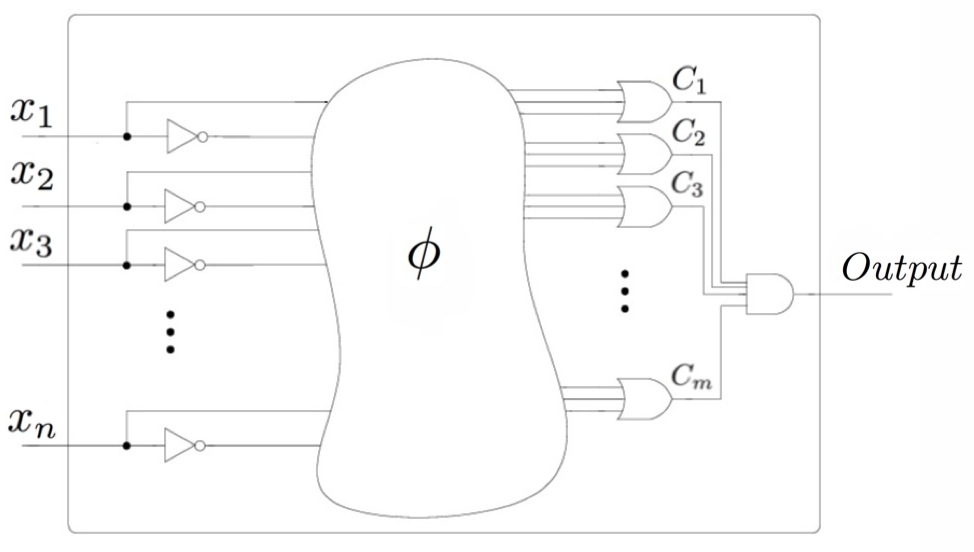
\includegraphics[width=0.9\textwidth]{figures/circuitLabeled.jpg}

\caption{A circuit describing {\sc Satisfiability}.}
\label{blackBoxSat}
\end{center}
\end{figure}
	
\FloatBarrier

%	<Paragraph> Provide complexity of {\sc Satisfiability}
The realization of {\sc Satisfiability} as a circuit reveals two aspects of this problem.  {\sc Satisfiability} can be implemented as a circuit with the number of gates proportional to the problem size.  The worst case verification for all $2^n$ possible witness candidates may be performed with the circuit in Figure \ref{blackBoxSat}.  This circuit consists of the hardware equivalent version of the {\sc Satisfiability} validator {\sc CheckSat}, as shown in Chapter 1.  
	
\section{Evaluating {\sc Sat} Solvers}

%	<Paragraph> Overview of evaluation
	
	In this section, we describe the standards for encoding the {\sc Satisfiability} problem that we adopt.  The standards come from from the {\sc Satisfiability} Competition \cite{dimacsFormat, satcompetition}.  
	
	Next, we introduce a problem instance classification scheme for {\sc Satisfiability}.  Classification of {\sc Satisfiability} problem instances include random, combinatorial, and industrial {\sc Sat} instances \cite{satcompetition}.  Our experiment in Chapter 6 generates random $k$-{\sc Sat} inputs.

	\subsection{Input and output}
	
%		<Paragraph> {\sc Satisfiability} standards [provide] common interface
	
%  Conforming to standards allows datasets and common interfaces to be shared.  
 The {\sc Sat} Competition ranks implementations of solvers for evaluating {\sc Satisfiability} \cite{satcompetition}.  {\sc Sat} solvers are evaluated on three categories of input: industrial, combinatorial, and random instances.  The input and output standards for {\sc Satisfiability} allow common benchmarks for {\sc Sat} solvers.  We conform to the standards of this competition \url{http://www.satcompetition.org/}.  
 

	
		\subsubsection{Input}
		
%			<Paragraph> DIMACS CNF [provides] standard benchmark instances
DIMACS CNF provides a standard input for {\sc Satisfiability} \cite{dimacsFormat}.  The format permits sharing of existing {\sc Satisfiability} benchmarks by encoding {\sc Satisfiability} in conjunctive normal form (CNF).  We provide an example of this encoding in Section \ref{inputSection}.
		
		\subsubsection{Output}
		
%			<Paragraph> Sat Competition output [provides] standard output

{\sc Sat} Competition output consists of the status of a DIMACS CNF input instance \cite{satcompetition}.  The status is provided for the instance as either \texttt{SATISFIABLE}, \texttt{UNSATISFIABLE}, or \texttt{UNKNOWN}.  If an instance can be determined as satisfiable, then a witness satisfying the instance gets included with the output status.  We provide an example along with custom output logging in Section \ref{outputSection}.
	
	\subsection{Metrics for classifying {\sc Satisfiability}}

%		<Paragraph> Describe metrics
{\sc Sat} phase transition and {\sc Sat} backbones are two metrics for classifying {\sc Satisfiability}.  We will use these metrics in the next section for defining a collection of random $k$-{\sc Sat} instances.
		
%		<Paragraph> {\sc Sat} phase transition


The ratio of $m$ clauses to $n$ variables $\alpha = m/n$ provides a characterization where phase transitions may occur in the space of all $k$-CNF formula \cite{Doherty08thehandbook,Gent94thesat}.  The {\sc Sat} phase transition is a region where both satisfiable and unsatisfiable instances are likely \cite{Gent94thesat}.  This region frequently separates trivially satisfiable and frequently over-constrained unsatisfiable {\sc Satisfiable} problem instances.  {\sc Satisfiability} instances with low $\alpha$ are frequently under-constrained and trivially satisfiable; those instances with high $\alpha$ are frequently over-constrained and trivially unsatisfiable \cite{Gent94thesat}.
		
%		<Paragraph> {\sc Sat} backbones
\begin{definition}
{\sc Sat} backbones are the variable assignments present in all of the satisfying assignments to a {\sc Satisfiability} problem instance \cite{Zhang2001}. 

\end{definition}

{\sc Sat} backbones contain a set of variables that occur in all satisfiable witnesses for an input instance.  If there are no such variables in the set of all witnesses for a problem instance, then the set is empty.

	\subsection{{\sc Satisfiability} instances}
		
%		<Paragraph> Various methods for [constructing] {\sc Satisfiability} instances
There are several methods for generating {\sc Satisfiability} instances.  We consider three classes \cite{satcompetition}: random assignment, combinatorial problems, and industrial applications.
	
\subsubsection{Random {\sc Sat}}
%		<Paragraph> {\sc Satisfiability} instance [generated] from random assignment
A random $k$-{\sc Sat} instance \cite{wilsonKsat}, for fixed $m$ and $n$, is one drawn uniformly from the set of all $k$-CNF formulas having $m$ clauses and $n$ variables.

%Random $k$-{\sc Sat} are generated with \texttt{ksat.c} \cite{wilsonKsat}.  A hash of the clause representation ensures that all clauses are independent \cite{wilsonKsat}.
%During generation of these formulas a hash is implemented to ensure that the random assignments ensure independent clauses and non-redundant variable assignments.  
		
%		<Paragraph> {\sc Satisfiability} instance [constructed] as hard assignment

\subsubsection{Hard combinatorial {\sc Sat}}

Combinatorial problem instances are well known difficult benchmark cases.  These instances include games and graph theoretic problems represented as {\sc Satisfiability}. 
		
%		<Paragraph> {\sc Satisfiability} instance [applied] from real world problems
\subsubsection{Industrial {\sc Sat}}

Industrial processes apply {\sc Satisfiability} to solve real world problems, including circuit layout, planning, logistics, circuit fault testing, and many other industrial \textsf{NP-complete} problems.  Industrial {\sc Sat} applications often apply heuristics and approximation techniques to relax the problem.  This allows approximate solutions to be computed efficiently with respect to time.
